\section{Question 2}
Used below equations to find the orbital elements.
$$
r = \begin{bmatrix}
    1600& 5310& 3800
\end{bmatrix}^{T}_{km}, \quad 
v = \begin{bmatrix}
    -7.35 & 0.46 & 2.47
\end{bmatrix}^{T}_{km/\sec}
$$
\subsection{part a}
$$
\boldsymbol h = \boldsymbol r \times \boldsymbol v 
$$
$$
v_r = \dfrac{\boldsymbol r \boldsymbol v}{r}
$$
$$
\boldsymbol e = \dfrac{\boldsymbol v \times \boldsymbol h -\mu \dfrac{\boldsymbol r}{r}}{\mu}
$$

$$
a = \dfrac{h^2}{\mu (1-e^2)}
$$

$$
\boldsymbol N = 
\begin{bmatrix}
    0 & 0 & 1
\end{bmatrix}^T \times \boldsymbol h
$$
$$
\theta = 
\begin{cases}
    \arccos\left(\dfrac{\boldsymbol e \cdot \boldsymbol r}{er}\right),& v_r >= 0\\
    2\pi-\arccos\left(\dfrac{\boldsymbol e \cdot \boldsymbol r}{er}\right),& v_r <  0\\
\end{cases}
$$

$$
\Omega = 
\begin{cases}
    \arccos\left(\dfrac{\boldsymbol N(1)}{N}\right),& \boldsymbol N(2) >= 0\\
    2\pi-\arccos\left(\dfrac{\boldsymbol N(1)}{N}\right) ,& \boldsymbol N(2) <0\\
\end{cases}
$$

$$
\omega = 
\begin{cases}
    \arccos\left(\dfrac{\boldsymbol N \cdot \boldsymbol e}{Ne}\right),& \boldsymbol e(3) >= 0\\
    2\pi-\arccos\left(\dfrac{\boldsymbol N \cdot \boldsymbol e}{Ne}\right) ,& \boldsymbol e(3) <0\\
\end{cases}
$$

$$
i = \arccos\left(\dfrac{\boldsymbol h(3)}{h}\right)
$$

From the above equations, initial conditions will find. The below equation shows the force of solar radiation.

$$
P_{SRP} = \nu \dfrac{S}{c}C_R \dfrac{A_s}{m}
$$
$\nu$ calculates if the satellite is in the earth's shadow or not.
Then used the below equations for rate changes.

\begin{equation*}
    \begin{split}
        \dfrac{dh}{dt} & = -p_{SR}ru_s \\
        \dfrac{de}{dt} & = -p_{SR} \left(\dfrac{h}{\mu} \sin(\theta)u_r+ \dfrac{1}{\mu h}\left((h^2+\mu r)\cos(\theta) \mu e r\right)u_s\right) \\
        \dfrac{d\theta}{dt} & = \dfrac{h}{r^2} - \dfrac{p_{SR}}{eh}\left(\dfrac{h^2}{\mu}\cos(\theta) u_r - \left(r+\dfrac{h^2}{\mu}\right)\sin(\theta)u_s\right) \\
        \dfrac{d\Omega}{dt} & = -p_{SR} \dfrac{r}{h\sin(i)}\sin(\omega + \theta)u_w\\
        \dfrac{di}{dt} & = -p_{SR} \dfrac{r}{h}\cos(\omega + \theta)u_w \\
        \dfrac{d\omega}{dt} & = -p_{SR} \left(\dfrac{1}{eh}\left(\dfrac{h^2}{\mu}\cos(\theta)u_r - \left(r+\dfrac{h^2}{\mu}\right)\sin(\theta)u_s\right)-\dfrac{r\sin(\omega - \theta)}{h\tan(i)}u_w\right)
    \end{split}
\end{equation*}
For this purpose, example 10.9 was used, the Gauss planetary equations for solar radiation pressure (Equations 10.106). The script file is Q2.m.

\begin{figure}[H]
    \caption{h changes in 5 years}
    \centering
    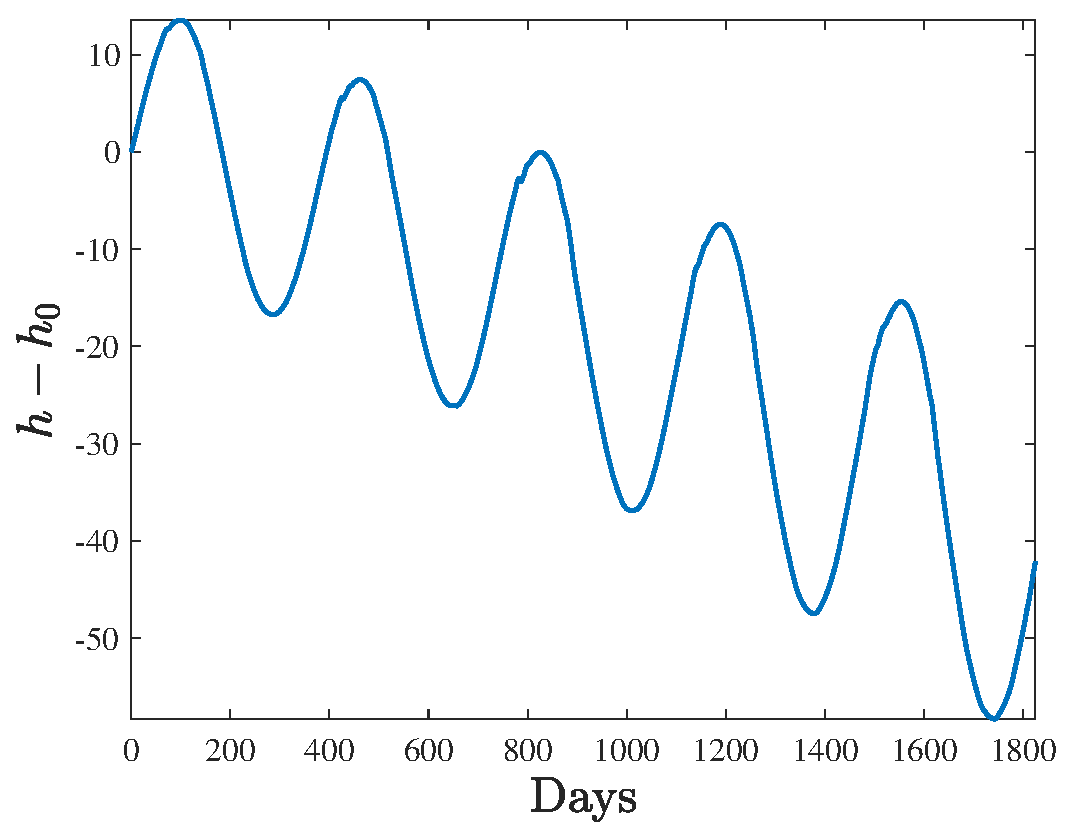
\includegraphics[width=12cm]{../Figure/Q2/h_fig}
\end{figure}

\begin{figure}[H]
    \caption{e changes in 5 years}
    \centering
    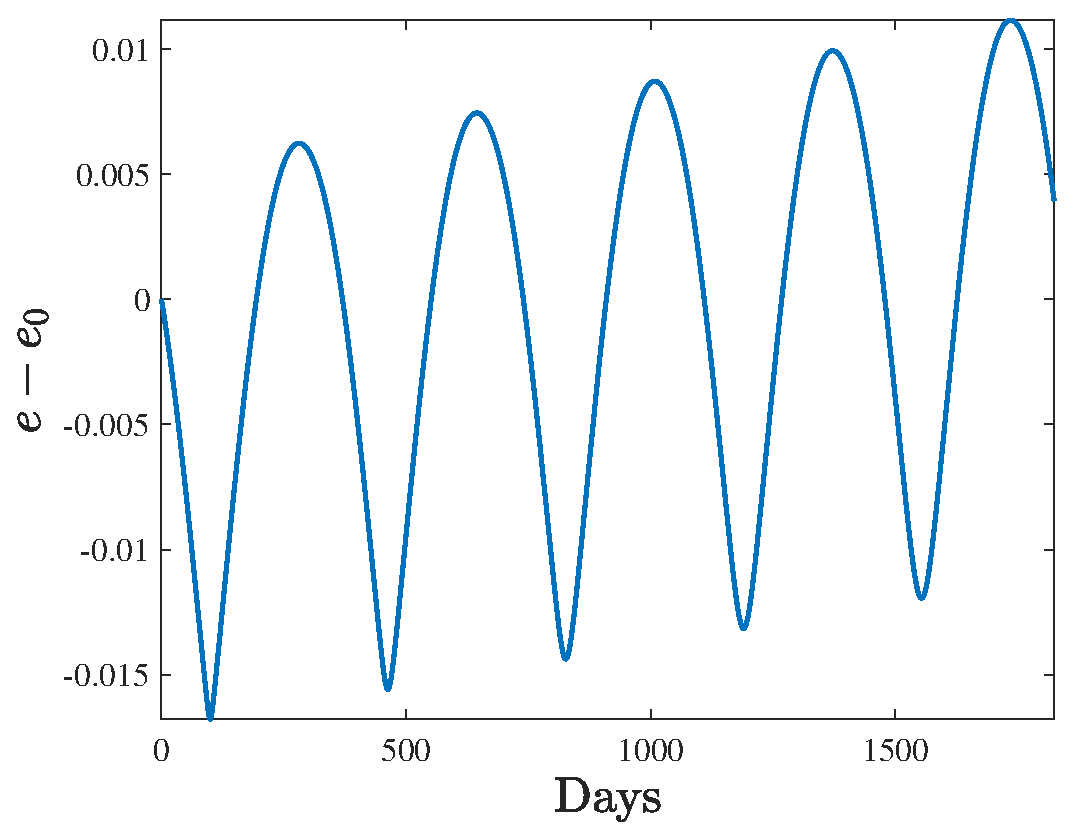
\includegraphics[width=12cm]{../Figure/Q2/e_fig}
\end{figure}

\begin{figure}[H]
    \caption{$\theta$ changes in 5 years (the satellite has a short period of 5 years of changes)}
    \centering
    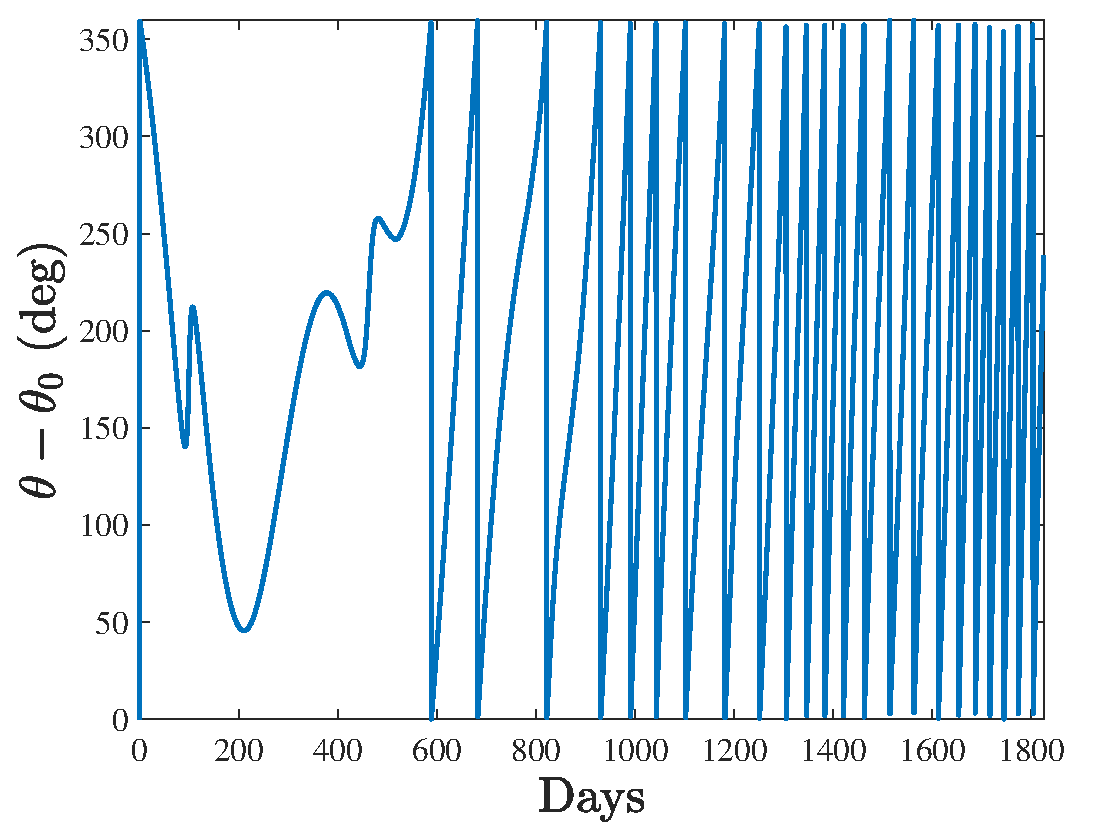
\includegraphics[width=12cm]{../Figure/Q2/theta_fig}
\end{figure}

\begin{figure}[H]
    \caption{$\Omega$ changes in 5 years (the satellite has a short period of 5 years of changes)}
    \centering
    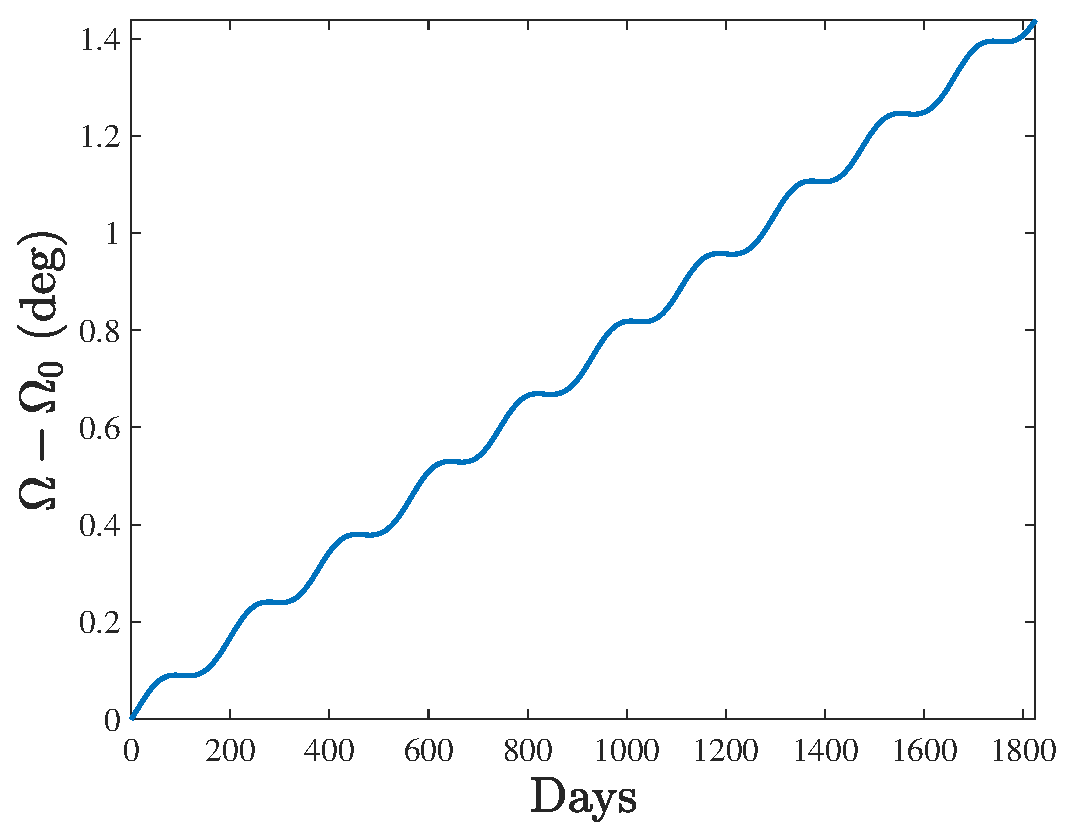
\includegraphics[width=12cm]{../Figure/Q2/Omega_fig}
\end{figure}

\begin{figure}[H]
    \caption{i changes in 5 years (the satellite has a short period of 5 years of changes)}
    \centering
    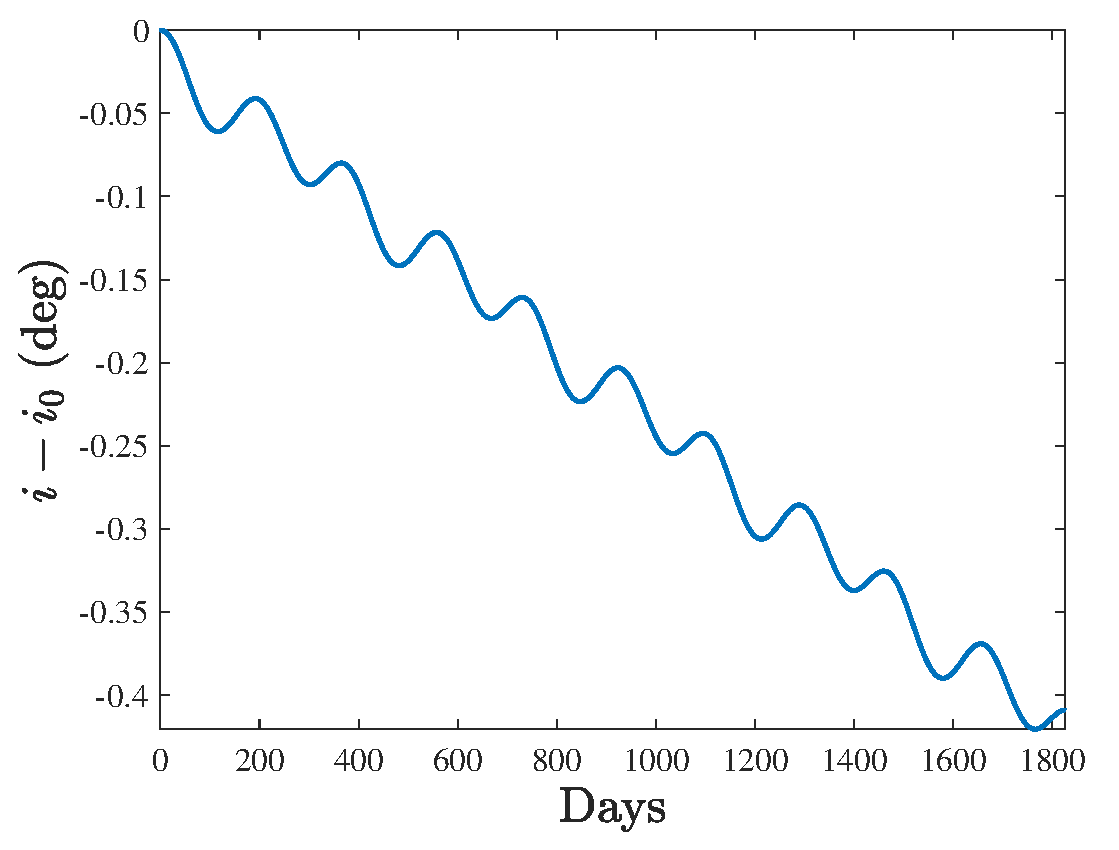
\includegraphics[width=12cm]{../Figure/Q2/i_fig}
\end{figure}

\begin{figure}[H]
    \caption{$\omega$ changes in 5 years (the satellite has a short period of 5 years of changes)}
    \centering
    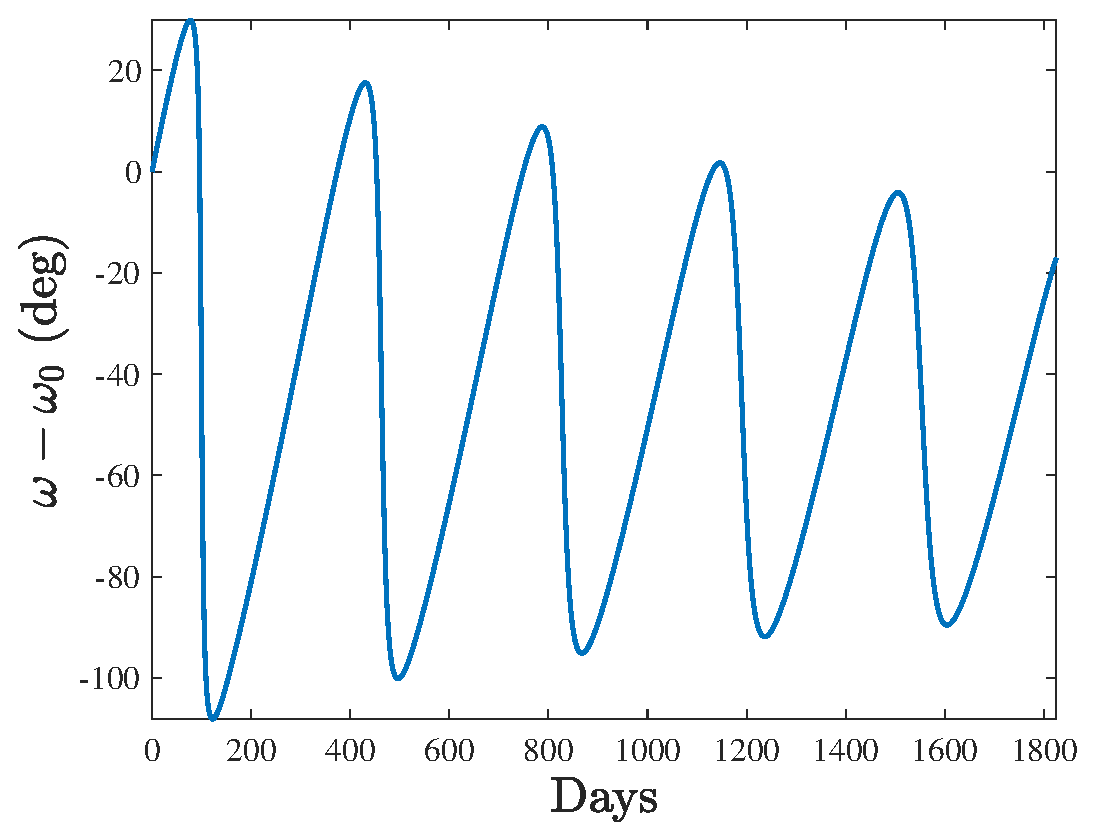
\includegraphics[width=12cm]{../Figure/Q2/omega_l_fig}
\end{figure}


\subsection{part b}
Used orbital elements from above code and sv\_from\_coe function from Curtis book to get satellite position and used Q1 short project to plot ground track.

\begin{figure}[H]
    \caption{Satellite latitude versus its longitude for one period}
    \centering
    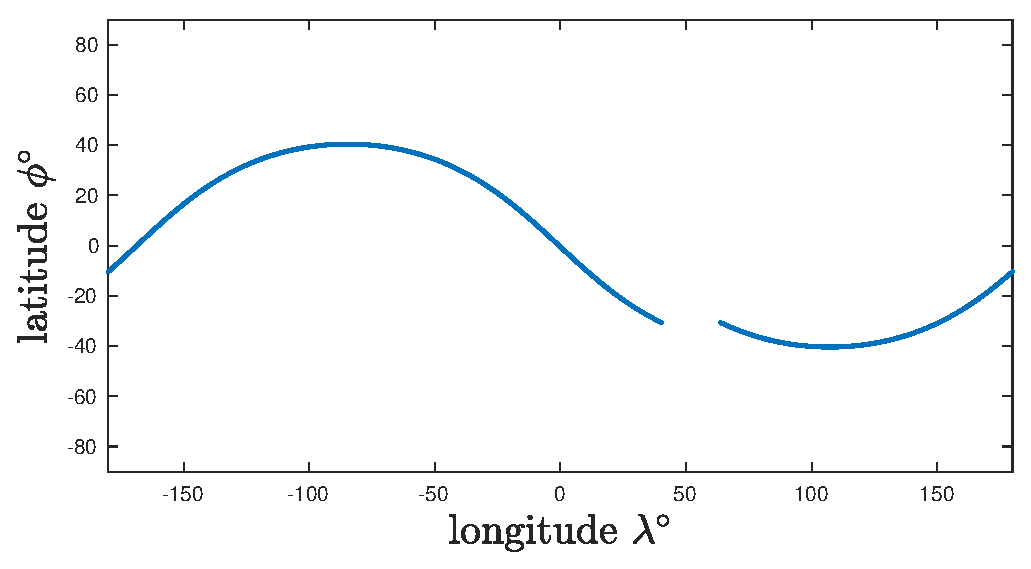
\includegraphics[width=16cm]{../Figure/Q2/latlong}
\end{figure}

Below the figure drawn provided by tamaskis, please click \href{https://github.com/tamaskis/ground_track-MATLAB}{here} to see the source code. Please use mentioned library to run code or skip part on earth fig.

\begin{figure}[H]
    \caption{Satellite latitude versus its longitude for one period}
    \centering
    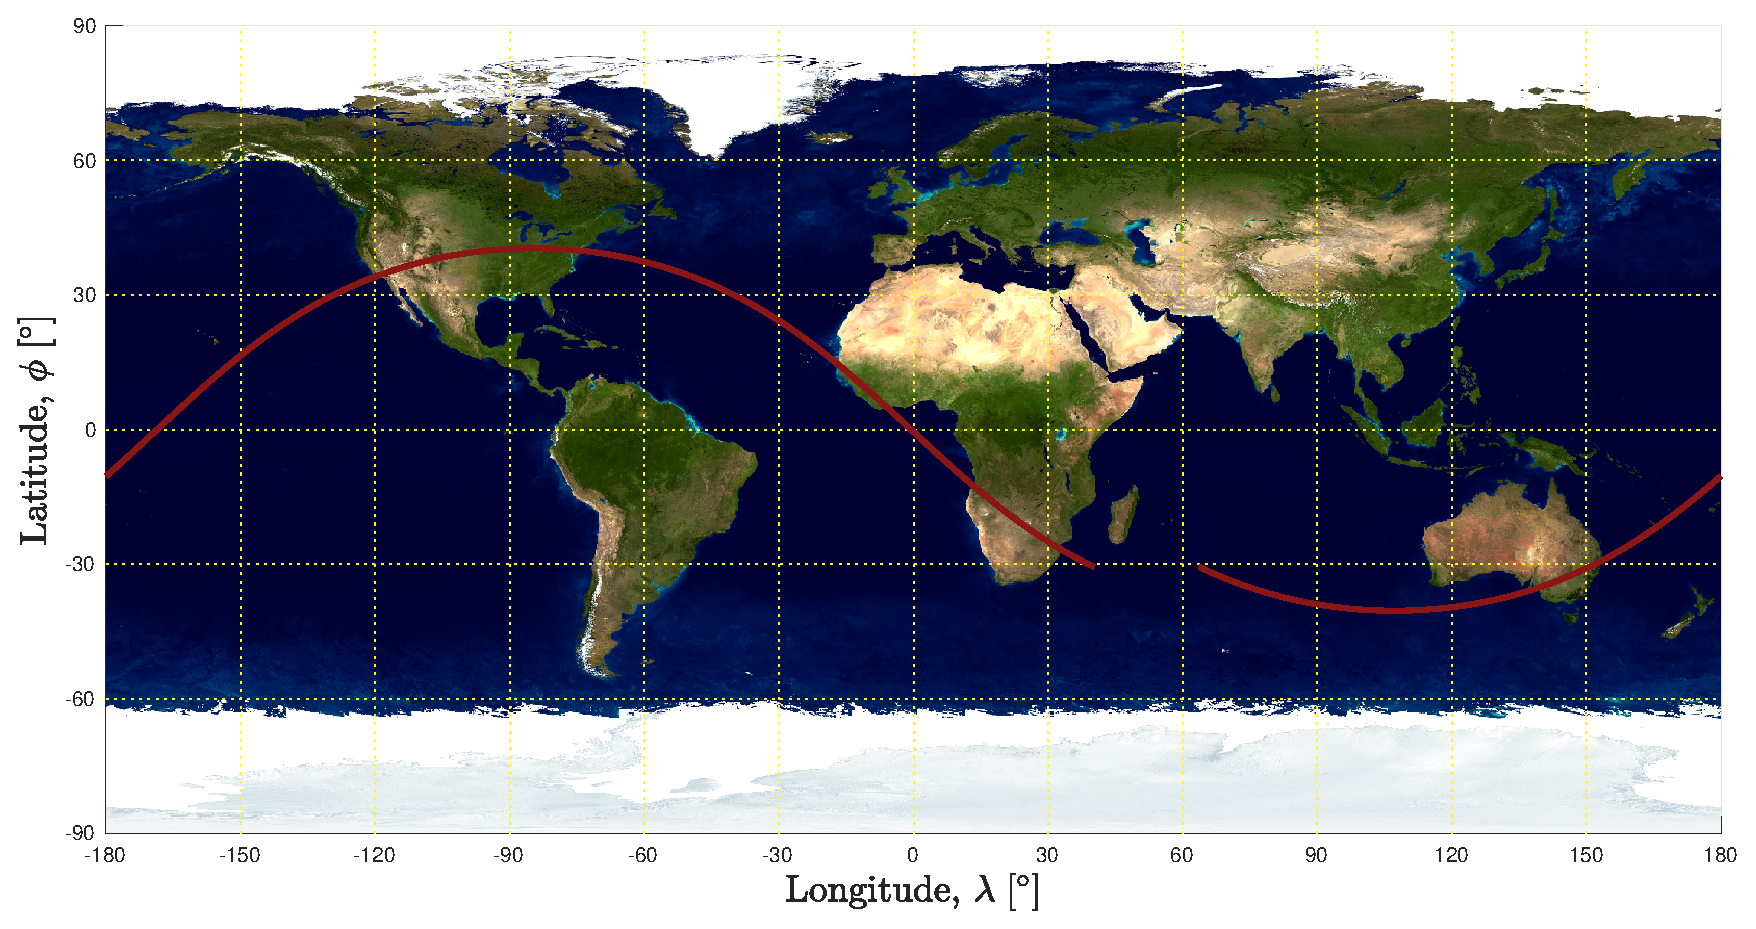
\includegraphics[width=16cm]{../Figure/Q2/latlong_earth}
\end{figure}

